Dieses Kapitel behandelt Methoden zur Generierung von diskreten und stetigen
mit beliebiger Verteilung Zufallszahlen. Wir nehmen an, mehrere
Pseudo-Zufallszahlengenerator (PRNG) $U_1, U_2, \ldots$ zur Verfügung zu haben,
die unabhängig voneinander $U(0,1)$ verteilte Zufallszahlen erzeugen.

PRNG sind nicht "`echt"' zufällig, da eine Folge von Zufallszahlen durch den
Startwert des Generators bestimmt ist und damit auch reproduziert werden kann.
Zusätzlich ist ein PRNG periodisch, sodass sich die generierten Zahlen ab einem
bestimmten Punkt wiederholen. Trotz dieser Eigenschaften sind (gute) PRNG sehr
gut für praktische Anwendungen geeignet, da sie sehr schnell Zufallszahlen
erzeugen können und die erzeugten Zahlen bei einem zufälligen Startwert nicht
von tatsächlich zufälligen Zahlen (z.B. bestimmt durch einen physikalischen
Prozess) unterscheidbar sind.

\section{Zufallszahlen mit diskreter Verteilung}

Ziel ist es, zufällig Zahlen zu erzeugen, die wie die Zufallsvariable $X$ mit
Zustandsraum $S = \{x_0, x_1, \ldots\}$ und zugehörigen Wahrscheinlichkeiten
$p_k = P(X=x_k)$ verteilt sind. Wir bestimmen im Folgenden ein Verfahren, mit
dem wir die Zufallszahlen $U_1\sim U(0,1)$ in die Zielverteilung umformen
können.

Das einfachste Vorgehen ist die proportionale Aufteilung des Intervalls $[0,1]$
gemäß der Wahrscheinlichkeiten $p_k$. Jedem $p_k$ wird der Bereich von $s_{k-1}$
bis $s_k$ zugewiesen, der genau $p_k$ breit ist:
\[
s_{k} = \sum_{i=0}^k p_k
\]
Fällt die von $U_1$ generierte Zufallszahl in das Intervall $(s_{k-1}, s_k)$, so
wird $x_k$ ausgegeben. Damit werden Zufallszahlen in der Zielverteilung erzeugt.

Folgender Algorithmus implementiert diese Methode und erzeugt $N$ wie $X$
verteilte Zufallszahlen:

\begin{algorithm}[h!]

\For{$1$ \KwTo $N$}{
  Setze $k=0$, $s=p_k$\;
  Erzeuge $u\sim U(0,1)$\;
  \While{$u > s$}{
    Setze $k \leftarrow k+1$\;
    Setze $s \leftarrow s+p_k$\;
  }
  Gib $x_k$ aus\;
}

\caption{Erzeugung diskreter Zufallszahlen}\label{algo:zz-diskret}
\end{algorithm}

Bei diesem Algorithmus sind in der inneren Schleife $\E(X)$ Durchläufe
notwendig (zumindest sofern $x_0 = 0$, $x_1=1$, usw. gilt)
um das $x_k$, in dessen Intervall $u$ fällt, zu finden.
Besitzt $X$ einen großen Zustandsraum, kann das die Geschwindigkeit des
Algorithmus erheblich verschlechtern.

Man kann die Laufzeiteigenschaften jedoch
verbessern, indem man $X$ auf eine Zufallsvariable $\hat{X}$ abbildet, deren
Werte $\hat{x}_k$ nach $\hat{p}_k$ absteigend geordnet sind. Somit steigt die
Wahrscheinlichkeit, bereits nach wenigen Durchläufen der inneren Schleife das
richtige $\hat{x}_k$ gefunden zu haben.

Die Idee hinter dem Algorithmus kann weiter verallgemeinert werden. Dafür
betrachten wir die \link{def:quantilf}{Quantilfunktion} von $X$, die die
\link{def:vertf-disk}{Verteilungsfunktion} umkehrt. Die Quantilfunktion gibt
uns also für Werte zwischen $0$ und $1$ zurück, was das $x_k$ zwischen $s_{k-1}$
und $s_k$ ist. Wir nutzen also (implizit) in Algorithmus \ref{algo:zz-diskret}
bereits die Quantilfunktion.

\begin{theorem}{Inversionsprinzip für diskrete Variablen}{invp}
Sei $X$ eine diskrete Zufallsvariable mit \link{def:vertf-disk}{Verteilungsfunktion}
$F_X$ und \link{def:quantilf}{Quantilfunktion}
$F_X^{-1}$. Weiterhin sei $U$ eine $U(0,1)$-verteilte Zufallsvariable. Dann
besitzt $F_X^{-1}(U)$ die gleiche Verteilung wie $X$, das heißt:
\[
P\big(F_X^{-1}(U)\le z\big) = F_X(z)
\]
\end{theorem}
Das ist die Formalisierung von unserem Ansatz, die Wahrscheinlichkeiten $p_k$
der Zufallsvariable $X$ proportional im Intervall $(0,1)$ zu betrachten.

\section{Inversionsmethode}\label{algo:inv-methode}

\begin{theorem}{Transformationssatz}{trafo}
Sei $X$ eine stetige Zufallsvariable mit \link{def:dichte}{Dichte} $\rho_X$ und
Zustandsraum $S$. Sind $a,b\in\R$ und $a \ne 0$, so besitzt die Zufallsvariable
$Y = a\cdot X + b$ die Dichte
\[
\rho_Y(z) = \rho_X\Big(\frac{z-b}{a}\Big)
\]
Ist die Funktion $g:S\to\R$ streng monoton, so hat die Zufallsvariable $Y=g(X)$
die Dichte
\[
\rho_Y(z) = \rho_X\big(g^{-1}(z)\big)\cdot\big|\big(g^{-1}\big)^\prime(z)\big|
\]
\end{theorem}

Die Wahrscheinlichkeitsdichte einer verteilte Zufallsvariable $Y$ kann auf die
Wahrscheinlichkeitsdichte einer anderen Zufallsvariable $X$ zurückgeführt
werden. Genau das wenden wir jetzt mit der Inversionsmethode an: Die
Zufallsvariable $Y$ soll eine beliebige Verteilung besitzten, die wir aus
gleichverteilten Zufallszahlen erzeugen. Dafür benötigen wir nur noch eine
geeignete Funktion $g$, sodass $Y=g(X)$ gilt. Das erreichen wir durch das
Inverse der Verteilungsfunktion:

\begin{theorem}{Inversionsmethode}{inversionsm}
Sei $U\sim U(0,1)$ eine gleichverteilte Zufallsvariable und $Y$ eine
beliebige stetige Zufallsvariable mit \link{def:vertf}{Verteilungsfunktion}
$F_Y$. Dann gilt:
\[
F_Y^{-1}(U) \sim Y
\]
\end{theorem}

\begin{example}{Exponentialverteilung}{exp}
Wir wollen Zufallszahlen $X\sim Exp(\alpha)$ erzeugen. $X$ besitzt die Dichte
\[
\rho(x) = \begin{cases}
\alpha \e^{-\alpha x} & x > 0 \\
0 & \text{sonst}
\end{cases}
\]
mit der Verteilungsfunktion
\[
F_X(z) = \begin{cases}
1- \e^{-\alpha z} & z > 0 \\
0 & \text{sonst}
\end{cases}
\]
Bei Einschränkung der Verteilungsfunktion auf den Zustandsraum $(0, \infty)$ von
$X$ ergibt sich:
\[
F_X: (0,\infty)\to(0,1):x\mapsto1-\e^{-\alpha x}
\]
Durch Umstellen ergibt sich folgende Vorschrift für die Umkehrfunktion:
\[
F_X^{-1}(y) = -\frac{1}{\alpha} \mathrm{ln}(1-y)
\]
Damit können wir mit der Inversionsmethode aus einer gleichverteilten
Zufallsvariable $U$ Zufallszahlen erzeugen, die wie $X$ verteilt sind:
\[
F_X^{-1}(U) = -\frac{1}{\alpha} \mathrm{ln}(1-U) \sim X
\]
\end{example}

Die Inversionsmethode ist ein effizientes Verfahren, um beliebig verteilte
Zufallszahlen zu erzeugen. Problematisch ist jedoch, dass wir die
Verteilungsfunktion invertieren müssen, was nicht immer möglich ist.

\section{Annahme-Verwerfungs-Methode}

\begin{wrapfigure}{r}{0.5\textwidth}
\centering
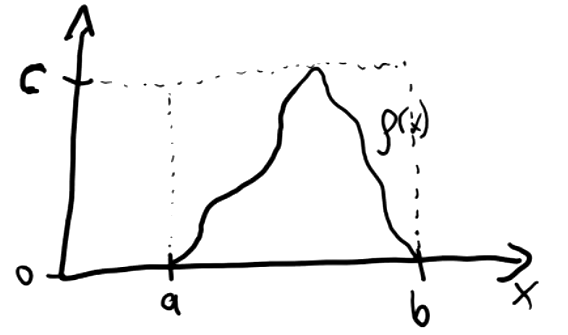
\includegraphics[width=0.4\textwidth]{av-methode}
\end{wrapfigure}
Die Annahme-Verwerfungs-Methode ist ein geometrischer Ansatz, der zufällig
Punkte in einem rechteckigen Bereich generiert, der die
\link{def:dichte}{Dichtefunktion} der gewünschten Verteilung einrahmt.
Notwendige Voraussetzung dafür ist, dass ein endlich großes, die Dichtefunktion
umgebendes Rechteck gefunden werden kann.

Die zufälligen Punkte werden durch skalierte, gleichverteilte Zufallszahlen
bestimmt. Liegt der Punkt unterhalb des Graphs der Dichtefunktion, wird der
X-Wert des Punkts ausgegeben. Damit entspricht die Wahrscheinlichkeit, dass ein
bestimmter Wert als Zufallszahl ausgegeben wird, genau dem Wert der
Wahrscheinlichkeitsdichte an diesem Punkt.

Der folgende Algorithmus gibt eine Folge von $N$ Zufallszahlen mit der gewünschten
Verteilung aus:

\begin{algorithm}[h!]

\For{$1$ \KwTo $N$}{
  Erzeuge $x\sim U(a,b)$\;
  Erzeuge $y\sim U(0,1)$\;
  \If{$y\cdot c \le \rho(x)$}{
    gib $x$ aus\;
  }
}

\caption{Annahme-Verwerfungs-Methode}\label{algo:av-methode}
\end{algorithm}

\subsection{Importance-Sampling}
\label{algo:imp-samp}

Die Annahme-Verwerfungs-Methode funktioniert dann besonders gut, wenn die Fläche
unter der Dichtefunktion im Vergleich zum einhüllenden Rechteck möglichst gering
ist. In diesem Fall liegen nur wenige Punkte oberhalb der Dichte und müssen
verworfen werden. Ist das einhüllende Rechteck im Vergleich jedoch sehr groß,
beispielsweise weil die Wahrscheinlichkeitsdichte sehr ungleich verteilt ist,
werden viele Punkte verworfen, sodass mehr Zeit für die Erzeugung einer festen
Anzahl an Zufallszahlen erforderlich ist.

Beim Importance-Sampling wird statt eines einhüllenden Rechtecks eine einhüllende
Funktion $h(x)$ verwendet, die weniger Platz als das Rechteck "`verschwendet"'.
Dafür ersetzen wir in Algorithmus \ref{algo:av-methode} die obere Schranke $c$
durch den Wert der Einhüllenden $h(x)$.

Da die Einhüllende $h(x)$ jedoch im Allgmeinen nicht konstant ist, müssen wir
diese Verzerrung korrigieren. Dafür generieren wir die x-Werte der zufälligen
Punkte in der Verteilung der Einhüllenden. Die Einhüllende $h(x)$ besitzt
folgende \link{def:dichte}{Dichte}:
\[H(z) = \frac{1}{\gamma}\cdot\int_a^z h(x) \mathrm{d}x\]
Die Konstante $\gamma = \int_a^b h(x)\mathrm{d}x$ stellt die Normiertheit sicher.

Durch die Inverse $H^{-1}$ der Verteilungsfunktion können mit der
\link{satz:inversionsm}{Inversionsmethode} der Einhüllenden entsprechend
verteilte Zufallszahlen erzeugt werden (da $h(x)$ frei gewählt werden kann, ist
das Invertieren in der Regel kein Problem).

Der entsprechende Algorithmus sieht dann so aus:

\begin{algorithm}[h!]

\For{$1$ \KwTo $N$}{
  Erzeuge $u\sim U(a,b)$\;
  Setze $x = H^{-1}(u)$\;
  Erzeuge $y\sim U(0,1)$\;
  \If{$y\cdot h(x) \le \rho(x)$}{
    gib $x$ aus\;
  }
}

\caption{Annahme-Verwerfungs-Methode mit Importance Sampling}\label{algo:av-methode-is}
\end{algorithm}

\section{Normalverteilte Zufallszahlen}

\begin{theorem}{Transformationssatz (2D)}{trafo-2d}
Seien $\zvec{X} = (X, Y)^\T$ und $\zvec{Z} = (S,T)^\T$
\link{def:zvektor}{Zufallsvektoren} mit gemeinsamer Dichte
$\rho_{X,Y}$ bzw. $\rho_{S,T}$. Weiterhin sei $g$ eine bijektive Funktion mit
Umkehrfunktion $g^{-1}$, die beide Zufallsvektoren aufeinander
abbildet:
\begin{align*}
g: \R^2\to\R^2: \begin{pmatrix}x\\y\end{pmatrix}\mapsto
  \begin{pmatrix}g_1(x,y)\\g_2(x,y)\end{pmatrix} =
  \begin{pmatrix}s\\t\end{pmatrix} \\
g^{-1}: \R^2\to\R^2: \begin{pmatrix}s\\t\end{pmatrix}\mapsto
  \begin{pmatrix}h_1(s,t)\\h_2(s, t)\end{pmatrix} =
  \begin{pmatrix}x\\y\end{pmatrix}
\end{align*}
Dann gilt für die Wahrscheinlichkeitsdichte von $\zvec{Z}$:
\[
\rho_{S,T}(s,t) = \rho_{X,Y}\big(g^{-1}(s,t)\big)\cdot\Det(J) =
  \rho_{X,Y}(h_1(s,t), h_2(s,t)) \cdot \Det(J)
\]
wobei $J$ die Jacobi-Matrix\more{wiki-jacobi} von $g^{-1}$ ist.
\end{theorem}

Ähnlich wie der \link{satz:trafo}{"`normale"' Transformationssatz} formalisiert der
2D-Tranformationssatz, wie sich die Wahrscheinlichkeitsdichte bei der Abbildung
einer Zufallsvariablen durch eine Funktion $g$ verändert. Das ist ein hilfreiches
Werkzeug bei der Erzeugung von Zufallszahlen, da wir im Allgemeinen
$U(0,1)$-verteilte Zufallszahlen in komplexere Verteilungen umformen möchten.

\subsection{Box-Muller-Methode}

Die Box-Muller-Methode nutzt den Transformationssatz und die Polardarstellung
von Koordinaten zur Erzeugung zweidimensional normalverteilter Zufallszahlen.

Seien $X\sim N(0,1)$ und $Y\sim N(0,1)$ \link{vert-stdnormal}{standardnormalverteilte}
und \link{def:zvar-unabh}{unabhängige} Zufallsvariablen. Damit bestehen folgende
Dichtefunktionen:
\begin{align*}
\rho_X(x) = \frac{1}{\sqrt{2\pi}}\cdot\exp\Big(-\frac{x^2}{2}\Big)\\
\rho_Y(y) = \frac{1}{\sqrt{2\pi}}\cdot\exp\Big(-\frac{y^2}{2}\Big)
\end{align*}
Da die Zufallsvariablen unabhängig sind, können wir Satz \ref{satz:randd}
anwenden um die gemeinsame Dichte zu bestimmen:
\[
\rho_{X,Y}(x,y) = \rho_X(x)\cdot\rho_Y(y) =
\frac{1}{2\pi}\cdot\exp\Big(-\frac{x^2+y^2}{2}\Big)
\]
Wir wenden den Transformationssatz mit einer Funktion $g$ an, die unsere
kartesischen Koordinaten $X,Y$ in Polarkoordinaten \more{wolfram-polar} $Z,\Phi$
umwandelt:
\begin{align*}
g: \R^2 \to \R^2: (x,y) &\mapsto (r^2 =x^2+y^2,\phi=\atan\frac{y}{x}) \\
g^{-1}: \R^2 \to \R^2: (z,\phi) &\mapsto (x=\sqrt{z}\cdot\cos\phi,y=\sqrt{z}\cdot\sin\phi)
\end{align*}
Dabei wird $z=r^2$ definiert. Als Jacobi-Matrix von $g^{-1}$ ergibt sich
\[
\renewcommand*{\arraystretch}{1.8}
J = \begin{pmatrix}\pd{h_1}{z} & \pd{h_1}{\phi} \\ \pd{h_2}{z} & \pd{h_2}{\phi}\end{pmatrix}
 = \begin{pmatrix}\frac{1}{2\sqrt{z}}\cos\phi & -\sqrt{z}\sin\phi \\
                  \frac{1}{2\sqrt{z}}\sin\phi &  \sqrt{z}\cos\phi\end{pmatrix}
\]
mit Determinante (Anwendung des trigonometrischen Pythagoras)
\[
\det J = \frac{1}{2}\cos^2\phi + \frac{1}{2}\sin^2\phi = \frac{1}{2}
\]
Durch Anwendung des \link{satz:trafo-2d}{Transformationssatzes} ergibt sich die
Verteilung $\rho_{Z,\Phi}$ der durch $g$ in Polarkoordinaten umgewandelten
Werte:
\begin{align*}
\rho_{Z,\Phi} &= \rho_{X,Y}(\sqrt{z}\cos\phi,\sqrt{z}\sin\phi)\cdot\det J \\
  &= \frac{1}{2\pi}\cdot
        \exp\Big(-\frac{(\sqrt{z}\cos\phi)^2+(\sqrt{z}\sin\phi)^2}{2}\Big)
        \cdot\det J \\
  &= \frac{1}{2\pi}\cdot\frac{1}{2}\exp\Big(-\frac{z}{2}\Big)
\end{align*}
Diese Verteilung besteht aus zwei bekannten Wahrscheinlichkeitsdichten: Der
erste Teil ist eine \link{vert-gleich}{Gleichverteilung} auf $(0,2\pi)$,
der zweite Teil ist eine \link{vert-exp}{Exponentialverteilung} mit
Parameter $\alpha=0.5$ (vgl. Beispiel \ref{bsp:exp}). Damit könnten wir
zweidimensional normalverteilte Zufallsvariablen erzeugen, wenn wir unabhängige
Zufallsvariablen $\Phi\sim U(0,2\pi)$ und $Z\sim Exp(0.5)$ erzeugen können.
Da wir annehmen, nur Zufallszahlen $U_1, U_2, ... \sim U(0,1)$ zur Verfügung zu
haben, wenden wir die \link{satz:inversionsm}{Inversionsmethode} an:
\begin{align*}
\Phi &= 2\pi \cdot U_1 \\
Z &= -2\ \ln(1-U_2)
\end{align*}
Durch Auflösung der Polarkoordinaten und $z = r^2$ erhält man:
\begin{align*}
X = \sqrt{-2\,\ln(1-U_2)}\cdot\cos(2\pi\cdot U_1) \\
Y = \sqrt{-2\,\ln(1-U_2)}\cdot\sin(2\pi\cdot U_1)
\end{align*}

Damit sind die Zufallsvariablen $X,Y \sim N(0,1)$ standardnormalverteilt. Um
$N(\mu, \sigma^2)$-verteilte Zufallsvariablen zu erzeugen, kann eine lineare
Transformation angewandt werden.

\medskip
Damit ergibt sich folgender Algorithmus zur Erzeugung von unabhängigen,
normalverteilten Zufallszahlen $X~N(\mu, \sigma^2)$. Der Algorithmus erzeugt
$N$ Paare von normalverteilten Zufallszahlen:

\begin{algorithm}[h!]

\For{$1$ \KwTo $N$}{
  Erzeuge $u\sim U(0,1)$\;
  Erzeuge $v\sim U(0,1)$\;
  Setze $z_1 = \sqrt{-2\,\ln(1-u)}\cdot\cos(2\pi\cdot v)$\;
  Setze $z_2 = \sqrt{-2\,\ln(1-u)}\cdot\sin(2\pi\cdot v)$\;
  Setze $x_1 = \sigma\cdot z_1 + \mu$\;
  Setze $x_2 = \sigma\cdot z_2 + \mu$\;
  Gib $x_1$ aus\;
  Gib $x_2$ aus\;
}

\caption{Box-Muller-Methode}\label{algo:box-muller}
\end{algorithm}

\subsection{Methode von Box, Muller, Marsaglia (Polarmethode)}

Die Polarmethode ist eine weitere Methode zur Erzeugung normalverteilter
Zufallszahlen, die die Auswertung von trigonometrischen Funktionen und des
Logarithmus vermeidet und daher schneller als die Box-Muller-Methode ist.

Der folgende Algorithmus beschreibt die Polarmethode:
\begin{algorithm}[h!]
\SetKw{Continue}{continue}

\For{$1$ \KwTo $N$}{
  Erzeuge $u\sim U(0,1)$\;
  Erzeuge $v\sim U(0,1)$\;
  Setze $x=2u-1$\;
  Setze $y=2v-1$\;
  Setze $s = x^2 + y^2$\;
  \If{$s\ge 1$}{
    \Continue
  }
  \eIf{$s \ne 0$}{
    Setze $z_1 = x\sqrt{\frac{-2\,\ln s}{s}}$\;
    Setze $z_2 = y\sqrt{\frac{-2\,\ln s}{s}}$\;
  }{
    Setze $z_1 = z_2 = 0$\;
  }
}

\caption{Box-Muller-Marsaglia-Methode (Polarmethode)}
\label{algo:box-muller-marsaglia}
\end{algorithm}

\section{Mehrdimensionale Zufallszahlen}

Bei der Erzeugung von Zufallsvektoren müssen die bedingte Abhängigkeiten
zwischen den jeweiligen Zufallsvariablen berücksichtigt werden.

Zufallsvektoren können in mehreren Schritten komponentenweise erzeugt werden.

Sei $\zvec{X} = (X,Y)^\T$ ein \link{def:zvektor}{Zufallsvektor} mit
\link{def:vert-zvektor}{Einzelwahrscheinlichkeiten} $p_{ij}$. Zuerst erzeugen
wir die erste Komponente des Vektors gemäß der \link{def:randv}{Randverteilung}
von $X$. Entsprechend dieser Verteilung wird mit einer geeigneten Methode
(Inversionsmethode, Annahme-Verwerfungs-Methode o.Ä.) ein $x$ ermittelt.

Durch die Randverteilung von $X$ können wir die \link{def:bedd}{bedingte
Einzelwahrscheinlichkeit} von $Y$, also $P(Y=y_i|x)$ bestimmt werden und ein
$y$ gemäß der Verteilung zufällig ermittelt werden.

Auf diese Weise können n-dimensionale Zufallszahlen erzeugt werden.

\subsection{Mehrdimensional normalverteilte Zufallszahlen}

\begin{figure}[h!]
\centering
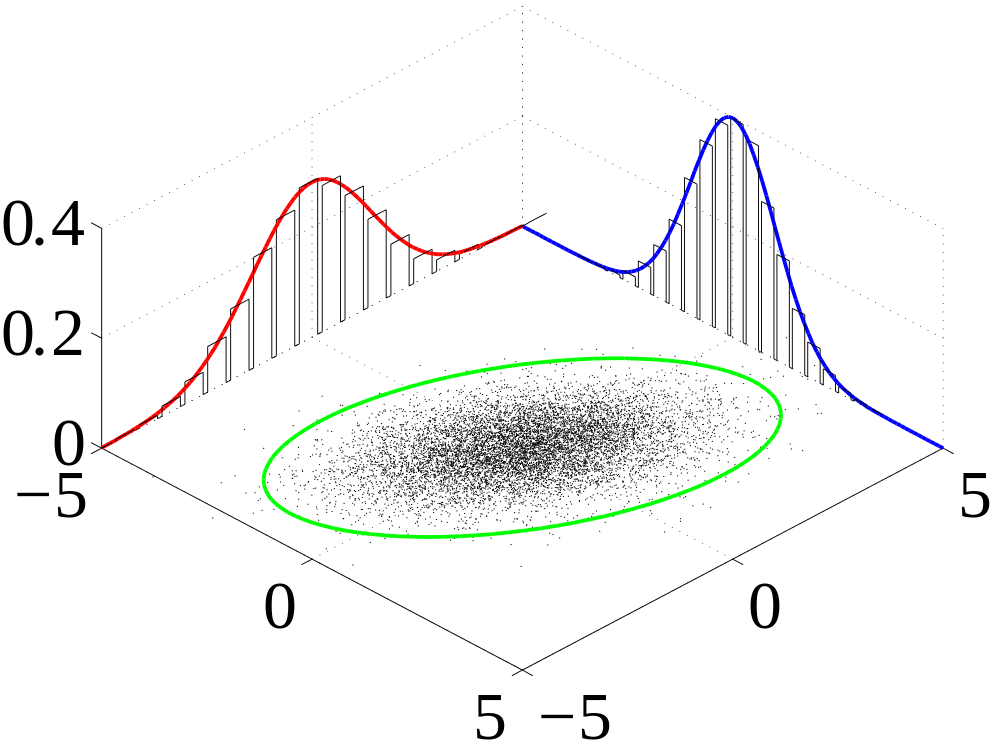
\includegraphics[width=10cm]{normal-2d}
\caption{Visualisierung einer zweidimensionalen Normalverteilung}
\end{figure}

\begin{definition}{Mehrdimensionale Normalverteilung}{ndim-normal}
Sei $\zvec{X} = (X_1, \ldots,X_d)^\T$ ein Zufallsvektor,
$\vec{\mu} = (\mu_1, \ldots, \mu_d)^\T \in\R^d$ ein Vektor der
Erwartungswerte und $\Sigma = (\sigma_{ij})_{i,j=1,\ldots,d}$
\link{def:kovarianz-matr}{Kovarianzmatrix} von $\zvec{X}$. Besitzt der
Zufallsvektor die Dichte
\[
\rho_{\zvec{X}} = \frac{1}{\sqrt{(2\pi)^d\cdot\det\Sigma}}\cdot
  \exp\Big(-\frac{1}{2}(\vec{x} - \vec{\mu})^\T\ \Sigma^{-1}(\vec{x}-\vec{\mu})\Big)
\]
so heißt er $\zvec{X}$ \defw{normalverteilt} (Schreibweise: $\zvec{X}\sim
N_d(\vec\mu,\Sigma)$). Jede Komponente des Vektors ist normalverteilt, das heißt
es gilt $\forall 0\le i\le d: X_i \sim N(\mu_i,\sigma_{ii})$.
\end{definition}

\begin{theorem}{Transformation einer mehrdimensionalen
Normalverteilung}{trafo-normal-ndim}
Sei $\zvec{X}$ ein normalverteilter Zufallsvektor von $d$ Komponenten mit
Erwartungswertvektor $\vec\mu$ und Kovarianzmatrix $\Sigma$. Sei $A$ eine
$n\times d$-Matrix ($n\in\N$). Dann ist die Transformation $\zvec{Y}= A\zvec{X}$
wieder normalverteilt mit
\begin{align*}
\E(\zvec{Y}) &= A\vec\mu \\
\Cov(\zvec{Y}) &= A\Sigma A^\T
\end{align*}
\end{theorem}

Diesen Satz können wir für die Erzeugung mehrdimensionaler Normalverteilungen
verwenden. Dafür erzeugen wir einen Zufallsvektor $\zvec{X} \sim
N_d(\vec{0},\mathds{1})$,
den wir so mit einer zu bestimmenden Matrix $A$ transformieren, dass gilt:
\[
\Cov(A\zvec{X}) = A\cdot \mathds{1}\cdot A^\T = A\cdot A^\T
\]

Dadurch ergibt sich folgender Algorithmus für die Erzeugung von $N$
wie $N_d(\vec\mu, \Sigma)$ verteilten Zufallsvektoren:
\begin{algorithm}[h!]

Finde $A\in\R^{(d\times d)}$ sodass $A\cdot A^\T = \Sigma$\;

\For{$1$ \KwTo $N$}{
  Erzeuge $z_1, \ldots,z_d$ unabhängig verteilt wie $N(0,1)$\;
  Setze $(x_1, \ldots, x_d)^\T = \vec\mu + A\cdot (z_1, \ldots, z_d)^\T$\;
  Gib $(x_1, \ldots, x_d)^\T$ aus\;
}

\caption{Erzeugung von normalverteilten Zufallsvektoren}
\label{algo:zz-normal-ndim}
\end{algorithm}

Um $z_1, \ldots, z_d$ zu erzeugen kann zum Beispiel die
\link{algo:box-muller-marsaglia}{Polarmethode} verwendet werden. Die Bestimmung
der Matrix $A$ entspricht der sogenannten Matrixwurzel von $\Sigma$, die durch
die Orthonormalbasis der Eigenvektoren bestimmt werden
kann\more{wiki-matrixwurzel}.
